% !TEX encoding = UTF-8 Unicode

\documentclass[a4paper]{article}

\usepackage{color}
\usepackage{url}
\usepackage[T2A]{fontenc} % enable Cyrillic fonts
\usepackage[utf8]{inputenc} % make weird characters work
\usepackage{graphicx}
\usepackage{amsfonts}

\usepackage[english,serbian]{babel}
%\usepackage[english,serbianc]{babel} %ukljuciti babel sa ovim opcijama, umesto gornjim, ukoliko se koristi cirilica

\usepackage[unicode]{hyperref}
\hypersetup{colorlinks,citecolor=green,filecolor=green,linkcolor=blue,urlcolor=blue}

%\newtheorem{primer}{Пример}[section] %ćirilični primer
\newtheorem{primer}{Primer}[section] %biće redefinisano kasnije


\begin{document}

\title{Vrste beskonačnosti. Paradoks Hilbertovog hotela\\ \small{Seminarski rad u okviru kursa\\Tehničko i naučno pisanje\\ Matematički fakultet}}

\author{Milica Zubljić\\ Branko Katanić\\ Dimitrije Spasojević\\ Luka Tonić\\ mi22047@alas.matf.bg.ac.rs}
\date{24.~oktobar 2017.} %biće ažuriran pre predaje rada
\maketitle

\abstract{
U ovom seminarskom radu biće govora o pojmu beskonačnosti. Objasnićemo šta je to beskonačnost, da li postoji više vrsta beskonačnosti, kako se interpretira beskonačnost u svakodnevnom životu itd. Ovaj interesantan koncept, kao i njegova (ne)pojmljivost ljudskom umu, biće ilustrovani kroz primer čuvenog paradoksa Hilbertovog beskonačnog hotela.\\

ključne reči: beskonačnost, prebrojivost, neprebrojivost
}

\tableofcontents %sadržaj

\newpage

\section{Uvod}
\label{poglavlje:uvod}

Svima nama dobro je poznat koncept beskonačnosti. U svakodnevnom razgovoru, ma o kojoj temi se razgovaralo, ovaj pojam se neretko javlja i ne iziskuje nikakvo objašnjavanje. No, da li možemo sa sigurnošću tvrditi da umemo da pojmimo taj opštepoznati koncept? Da li je pojam beskonačnosti jednoznačan ili, pak, ima potrebe precizirati njegovo značenje? Odgovore na ova pitanja naći ćete u nastavku teksta.

\section{Nešto o beskonačnostima}
\label{poglavlje:Nešto o beskonačnostima}

Prva istraživanja pojma beskonačnosti otpočela su još vekovima pre nove ere. Ovim pojmom bavili su se žitelji Starog Egipta i Stare Grčke, kolevke moderne kulture. Jedan od prvih ljudi zainteresovanih za taj pojam bio je čuveni antički filozof Zenon iz Eleje. \cite{Zenon} U filozofiji, beskonačno je ono što je neograničeno, što ide izvan bilo koje utvrdjene granice.\\

Kada biste pitali decu koji je najveći broj koji postoji, verovatno bi vam rekla: beskonačno. Ako posmatramo problem na taj način, mogli biste im odvratiti da je broj veći od beskonačno: beskonačno plus jedan. Tako možemo ići u nedogled, ali poenta je da u matematici beskonačno \textbf{nije brojevna vrednost}. Ona zapravo označava nešto što nije konačno, nešto veoma veliko. Ako uzmemo za primer neku promenljivu, ona ne može biti jednaka beskonačnosti, ali može joj težiti. U tom kontekstu, pojam beskonačnosti koristi se u radu sa limesima, integralima, geometrijskim redovima itd.\\


\subsection{Zanimljivosti}

\begin{itemize}
    \item Simbol beskonačnosti '$\infty$' uveo je britanski matematičar Džon Volis (eng. John Wallis) u 17. veku. Taj simbol nastao je po uzoru na stari zapis rimskog broja hiljadu, koji je takodje označavao neki veoma veliki broj. (slika \ref{fig:Uzor za simbol beskonačnosti danas})
    
    \begin{figure}[ht!]
    \begin{center}
    
\includegraphics[scale=0.75]{sablon_za_seminarski_rad/Simbol.PNG}
    \end{center}
    \caption{Uzor za simbol beskonačnosti danas}
    \label{fig:Uzor za simbol beskonačnosti danas}
    \end{figure}
    
    \item U alhemiji, grani filozofije prirode iz koje su se razvile moderne nauke kao što su hemija i farmakologija, beskonačnost je predstavljao Uroboros, zmaj sa repom u ustima koji neprestano proždire samog sebe. (slika \ref{fig:Uroboros})
    
    \begin{figure}[ht!]
    \begin{center}
    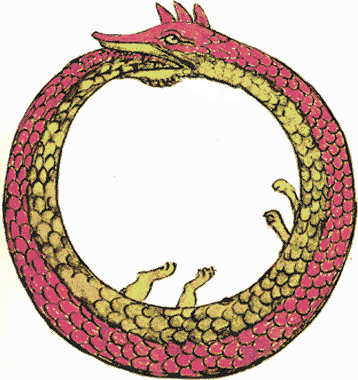
\includegraphics[scale=0.4]{sablon_za_seminarski_rad/Uroboros.png}
    \end{center}
    \caption{Uroboros}
    \label{fig:Uroboros}
    \end{figure}
\end{itemize}

\newpage

\section{Kardinalnost skupa. Pojam prebrojivosti}
\label{poglavlje:Kardinalnost. Pojam prebrojivosti}

%Za neki skup kažemo da je prebrojiv ako postoji bijekcija f sa skupa prirodnih brojeva u taj skup.
%Drugim rečima, skup je prebrojiv ako se njegovi članovi mogu poredjati u niz.

Znamo da postoje brojevni skupovi koji nemaju konačan broj elemenata. Takvi su osnovni skupovi kojima rukujemo u matematici: prirodni, celi, racionalni, iracionalni i realni brojevi.

Nama najintuitivniji od njih jeste skup prirodnih brojeva ($\mathbb{N}$). U teoriji, možemo početi da brojimo od 1 pa nadalje (2,3,4,...) i da budemo sigurni da nijedan broj nismo preskočili u procesu, iako taj proces nema kraja. Tako bismo naveli sve prirodne brojeve (za beskonačno dug vremenski period). Slično tome, možemo brojati od 0 naniže i pokriti skup celih brojeva ($\mathbb{Z}$). Kod skupa racionalnih brojeva ($\mathbb{Q}$) malo je kompleksniji postupak \cite{Kantorov dijagonalni postupak}, ali njegovom primenom takodje možemo biti sigurni da nijedan broj nismo ispustili.

Pošto članove navedenih skupova možemo poredjati u niz iako ih ima beskonačno mnogo, kažemo da oni imaju \textbf{prebrojivo mnogo} elemenata. Formalnije, za neki skup kažemo da je prebrojiv ako postoji bijekcija $f$ sa skupa prirodnih brojeva u taj skup.

Dakle, govorimo o \textbf{prebrojivoj beskonačnosti}. Ona se u matematici obeležava sa $\aleph_{0}$ ($\aleph$ - prvo slovo hebrejske azbuke).\\

S druge strane, govoreći o skupovima iracionalnih ($\mathbb{I}$) i realnih ($\mathbb{R}$) brojeva, ne postoji metoda kojom bismo njihove elemente mogli poredjati u niz i sve ih nabrojati. Zato kažemo da ovakvi skupovi imaju \textbf{neprebrojivo mnogo} elemenata i govorimo o \textbf{neprebrojivoj beskonačnosti}. Više o tome u nekom od sledećih poglavlja.


\section{Hilbertov hotel. Konačan broj novih gostiju}
U 19. veku Georg Kantor je uveo pojam kardinalnosti i prebrojivosti skupova. Njegova teorija naišla je na mnogo osuda tadašnjih cenjenih matematičara.
Jedan od ljudi koji je ipak prepoznao njen značaj bio je David Hilbert.
On je uspeo da nam vrlo slikovito približi pojam beskonačnosti, opisavši problem smeštanja beskonačno mnogo gostiju u hotel sa beskonačno mnogo soba - \textbf{Hilbertov hotel.}
Hilbertov hotel je hotel koji ima beskonačno mnogo soba i sve su popunjene. Da li u njega ipak može stati jos gostiju?

\subsection{Konačan broj novih gostiju}
Dakle, ispred potpuno punog hotela nalazi se jedan gost koji traži sobu. Kako rešiti ovaj problem?
Novu sobu možemo osloboditi ako zamolimo gosta iz sobe 1 da predje u sobu 2, gosta iz sobe 2 u sobu 3 i tako dalje. Dakle, gost iz sobe \textit{n} prelazi u sobu \textit{n+1}.
Pošto na raspolaganju imamo beskonačan broj soba, za svaku sobu \textit{n} će postojati soba \textit{n+1}, pa ćemo lako smestiti sve goste u nove sobe i tako osloboditi sobu broj 1.
Ovaj isti postupak može se primeniti na bilo koji konačan broj gostiju. Na primer, ako treba osloboditi 100 novih soba, svakog gosta ćemo premestiti iz svoje sobe u sobu čiji je broj za 100 veći.
Na malo komplikovaniji problem nailazimo kada na red ne čeka konačan broj gostiju.

\newpage
\section{Beskonačan broj gostiju. Pojam prebrojivosti}
\label{sec:beskonačan broj gostiju}
Pred hotelom se sada nalazi beskonačno veliki autobus sa \textbf {prebrojivo} beskonačno mnogo putnika.a
U našem primeru Hilbertovog hotela, jasno je da je činjenica da gostiju ima \textbf {prebrojivo} mnogo ključna ako hocemo da ih rasporedimo po sobama.
Ovaj problem možemo rešiti tako što ćemo gosta iz prve sobe zamoliti da predje u drugu, gosta iz druge u četvrtu, iz treće u šestu i tako dalje.
Uopšteno, gost iz sobe \textbf {n} prelazi u sobu \textbf {2n}. Ovim procesom smo oslobili sve sobe sa neparnim brojem.
Pošto neparnih brojeva ima beskonačno mnogo, to ostavlja dovoljno mesta za sve putnike beskonačno velikog autobusa.

\subsection {Dokaz o beskonačnosti skupa neparnih brojeva}
Pretpostavimo suprotno, to jest da je skup neparnih brojeva konačan.
To znači da postoji najveći broj \textit{n} iz tog skupa.
Svaki neparni broj možemo zapisati u obliku \textit{2p+1}, gde je \textit{p} bilo koji ceo broj, pa tako možemo zapisati i ovaj najveći broj.
Sada razmatrajmo broj \textit{n+2}. \textit{n+2=2p+1+2=2(p+1)+1}.
Broj \textit{2(p+1)} očigledno je paran, pa zaključujemo da je broj \textit{n+2} neparan, a u isto vreme veći od najvećeg neparnog broja.
Ovim zaključkom dolazimo do kontradikcije, što znači da smo dokazali da neparnih brojeva ima beskonačno mnogo.




\newpage

\section{Kako smestiti beskonačno ljudi iz beskonačno autobusa u hotel}
\label{poglavlje:Kako smestiti beskonačno ljudi iz beskonačno autobusa u hotel}
Jedne noći, dešava se nezamislivo. Noćni poslovođa gleda napolje i vidi beskonačnu kolonu beskonačno velikih autobusa, svaki sa prebrojivo beskonačnim brojem putnika. Ako ne nađe sobe za njih, hotel će izgubiti beskonačnu sumu novca, a on će sigurno izgubiti posao. Srećom, seti se da je oko 300. godine p.n.e Euklid dokazao da postoji beskonačan broj prostih brojeva. Da bi ispunio ovaj naizgled nemoguć zadatak da nađe beskonačan broj kreveta za beskonačne autobuse, pune umornih putnika u beskonačnom broju, noćni poslovođa dodeljuje svakom već postojećem gostu prvi prost broj, 2, stepenovan brojem njihove sobe. Tako gost iz sobe broj 7 odlazi u sobu broj $2^7$, a to je soba 128. Poslovođa zatim uzima ljude iz prvog od beskonačnih autobusa i dodeljuje im sobu broj: sledeći prost broj, 3, stepenovan brojem njihovog sedišta u autobusu. Tako osoba na sedištu broj 7 u prvom autobusu odlazi u sobu broj $3^7$ to jest u sobu 2.187. To se nastavlja za ceo prvi autobus. Putnicima iz drugog autobusa se dodeljuju eksponenti sledećeg prostog broja, 5. Sledećem autobusu, eksponenti broja 7. Sledećim autobusima: eksponenti broja 11, eksponenti broja 13, broja 17 i tako dalje.


\subsection{Euklidov dokaz, Beskonačno prostih brojeva}
Neka je dat bilo koji konačni skup prirodnih brojeva p1, p2, ..., pn. Biće pokazano da postoji barem još jedan prost broj koji se ne nalazi u listi. Neka je P proizvod svih prostih brojeva u skupu: P = p1p2...pn. Neka je q = P + 1. Tada q ili jeste ili nije prost broj:
\begin{itemize}
\item Ako je q prost, onda postoji bar jedan broj (q) koji je prost, a nije u prvobitnom skupu.
\item Ako q nije prost, onda neki prost broj p deli q. Kad bi ovaj broj p bio u skupu, tada bi on delio P (jer je P proizvod svih brojeva u skupu); ali p deli P + 1 = q. Ako p deli P i q, onda bi p morao da deli razliku
\cite{objasnjenje_deljenja} ova dva broja, što je (P + 1) - P ili jednostavno 1. Kako nijedan prost broj ne deli 1, p ne može biti u skupu. Ovo znači da barem još jedan prost broj mora postojati mimo onih koji su već u skupu.
\end{itemize} 

Ovo dokazuje da za svaki konačni skup prostih brojeva postoji prost broj koji nije u tom skupu, i stoga prostih brojeva mora biti beskonačno mnogo.


\addcontentsline{toc}{section}{Literatura}
\appendix

\iffalse
\bibliography{seminarski} 
\bibliographystyle{plain}
\fi

\renewcommand{\refname}{Literatura}
\begin{thebibliography}{9}


\end{thebibliography}


\addcontentsline{toc}{section}{Dodatak: objašnjenja}
\renewcommand{\refname}{Dodatak: objašnjenja}
\begin{thebibliography}{9}

\bibitem{Zenon} Zenon (Eleja, 490-430. g.p.n.e.) - grčki filozof, pripadnik elejske škole koju je osnovao Parmenid

\bibitem{Kantorov dijagonalni postupak} Tabela čije su prva vrsta ($p$) i prva kolona ($q$) prirodni brojevi (1,2,3,...). U presecima odgovarajućih vrsta i kolona dobijaju se racionalni brojevi oblika $\frac{p}{q}$, a nabrajaju se po dijagonalama ($\frac{1}{1}, \frac{2}{1}$, $\frac{1}{2}$, $\frac{1}{3}$, $\frac{2}{2}$, $\frac{3}{1}$,...)

\bibitem{objasnjenje_deljenja}U opštem slučaju, za svaka tri cela broja a, b, c ako $a \mid b$ i $a \mid c$ onda $a \mid (b - c)$.





\end{thebibliography}


\end{document}